% 需要在导言区加载：\usepackage{graphicx,booktabs,float}

\begin{figure}[H]
  \centering
  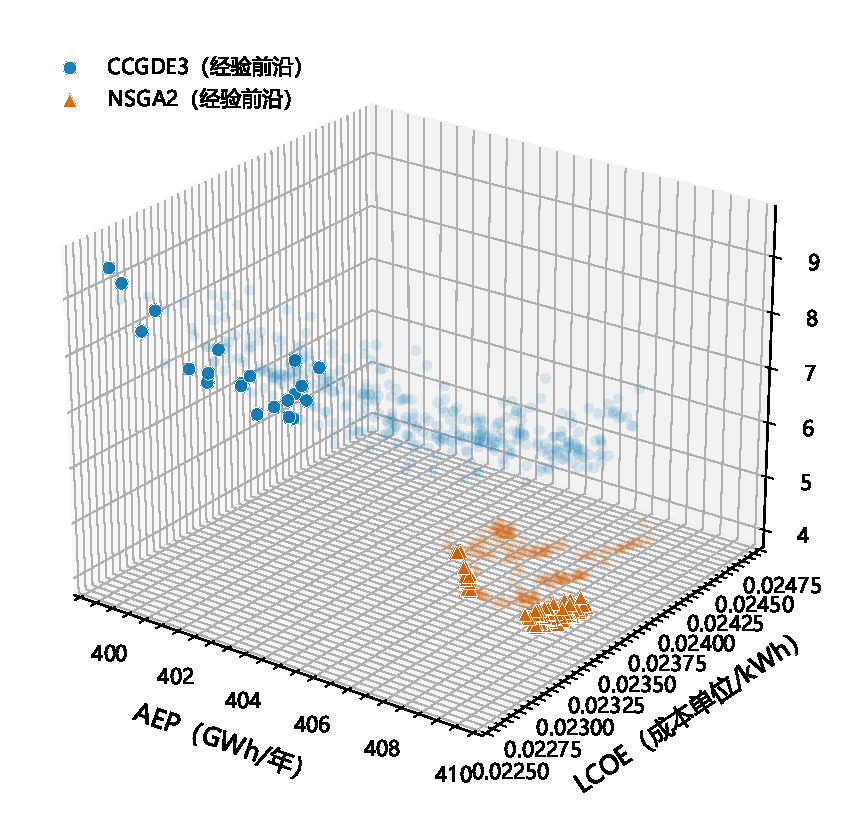
\includegraphics[width=0.86\textwidth]{图表/fig_pareto_front.pdf}
  \caption{两种算法的三目标最终解集与合并经验 Pareto 前沿。浅色点为所有最终档案解，实色点为合并后的非支配解。}
  \label{fig:pareto-front}
\end{figure}

\begin{figure}[H]
  \centering
  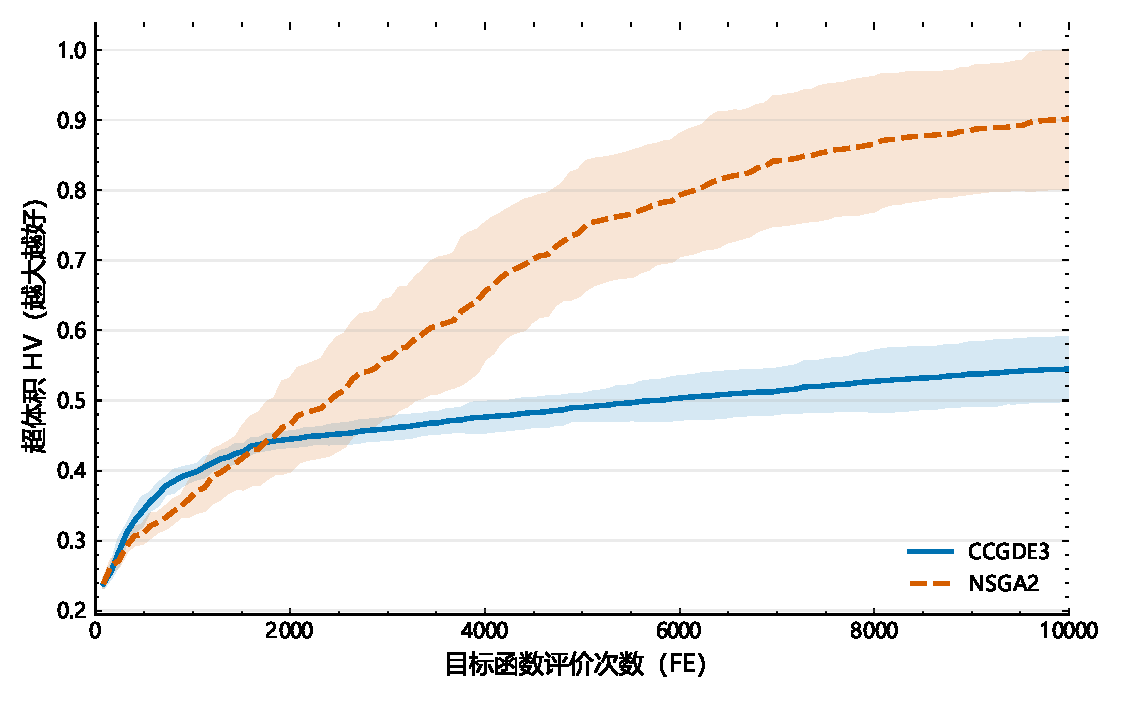
\includegraphics[width=0.82\textwidth]{图表/fig_convergence_hv.pdf}
  \caption{HV 随目标函数评价次数的收敛过程。实线为 5 次运行的均值，阴影为均值$\pm$1 倍标准差。}
  \label{fig:convergence-hv}
\end{figure}

\begin{figure}[H]
  \centering
  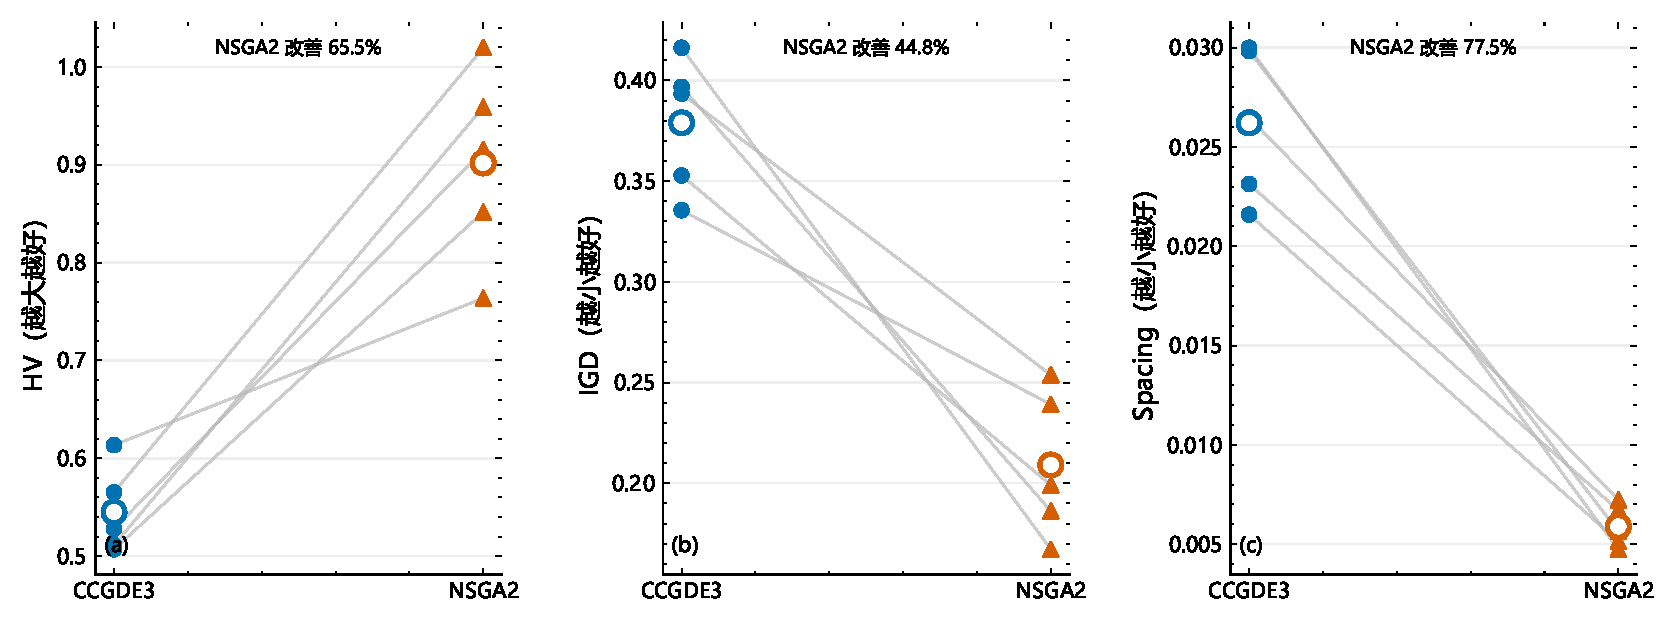
\includegraphics[width=\textwidth]{图表/fig_metric_distribution.pdf}
  \caption{5 个相同随机种子下 HV、IGD 和 Spacing 的配对对比。连线表示同一随机种子，空心大点表示均值。}
  \label{fig:metric-distribution}
\end{figure}

\begin{figure}[H]
  \centering
  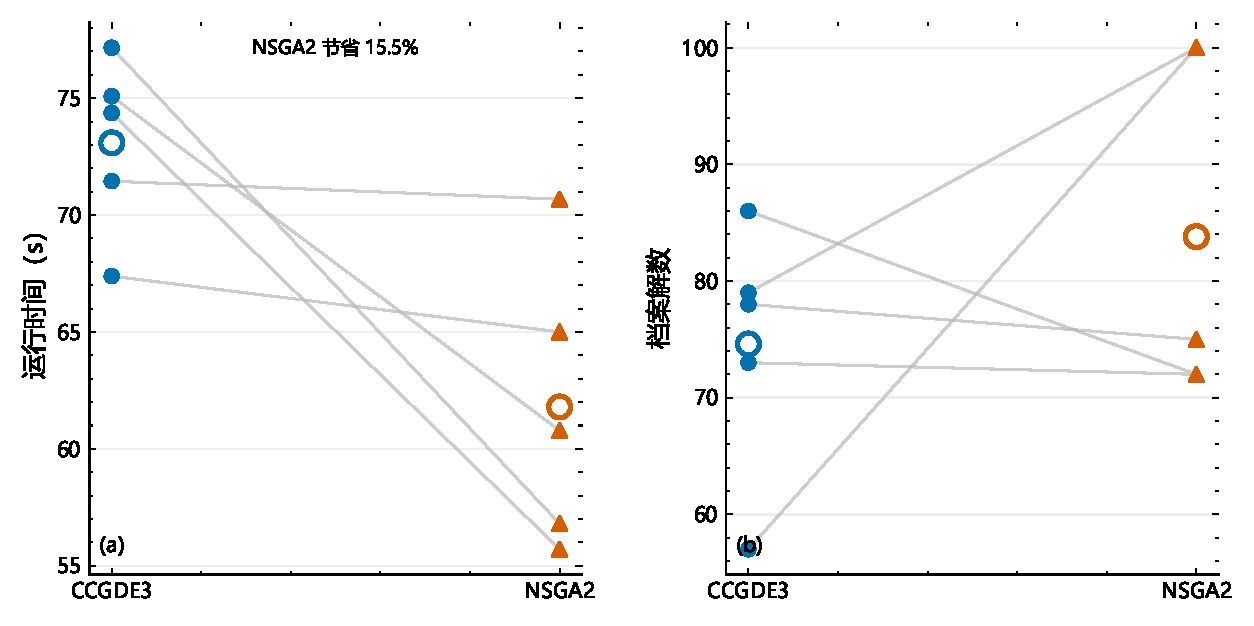
\includegraphics[width=0.88\textwidth]{图表/fig_runtime.pdf}
  \caption{两种算法的运行时间与最终档案解数配对对比。}
  \label{fig:runtime}
\end{figure}

\begin{figure}[H]
  \centering
  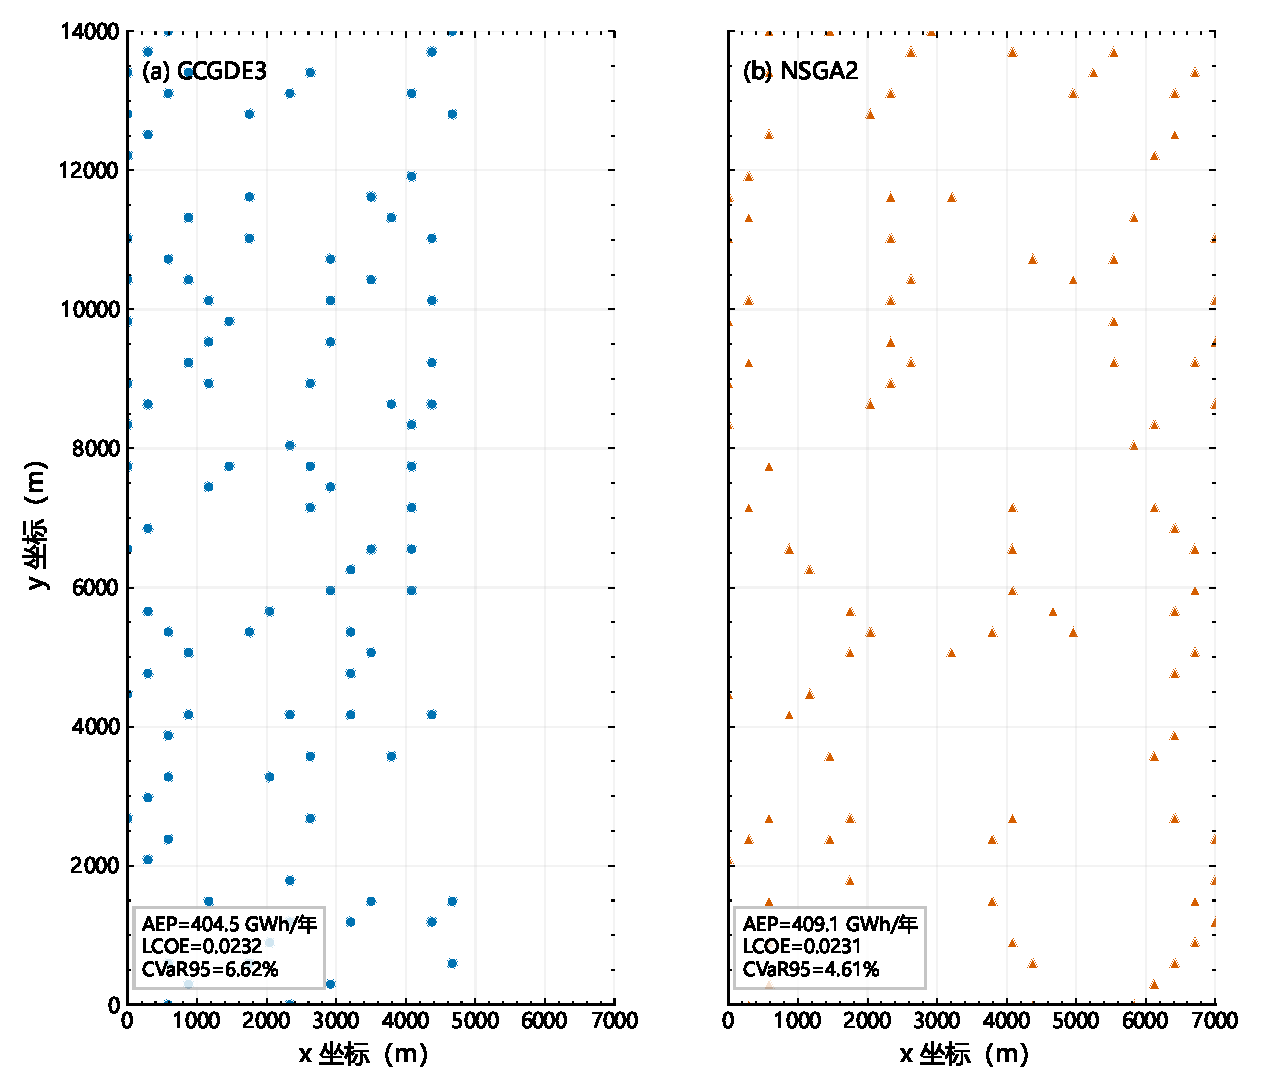
\includegraphics[width=0.88\textwidth]{图表/fig_layouts.pdf}
  \caption{两种算法代表性折中解的 100 台风机空间布局。}
  \label{fig:representative-layouts}
\end{figure}

\begin{table}[H]
\centering
\caption{两种算法的综合性能对比（5 个配对随机种子）}
\label{tab:algorithm-comparison}
\resizebox{\textwidth}{!}{%
\begin{tabular}{lccccc}
\toprule
指标 & CCGDE3（均值$\pm$标准差） & NSGA2（均值$\pm$标准差） & NSGA2 改善幅度 & 配对胜场 & 单侧符号检验 $p$ \\
\midrule
HV（$\uparrow$）       & $0.5450\pm0.0447$ & $0.9018\pm0.0986$ & $+65.48\%$ & $5/5$ & 0.03125 \\
IGD（$\downarrow$）    & $0.3790\pm0.0335$ & $0.2091\pm0.0363$ & $-44.83\%$ & $5/5$ & 0.03125 \\
Spacing（$\downarrow$）& $0.02621\pm0.00382$ & $0.00590\pm0.00105$ & $-77.50\%$ & $5/5$ & 0.03125 \\
运行时间/s（$\downarrow$） & $73.09\pm3.79$ & $61.79\pm6.17$ & $-15.46\%$ & $5/5$ & 0.03125 \\
档案解数 & $74.6\pm10.9$ & $83.8\pm14.8$ & $+12.33\%$ & -- & -- \\
\bottomrule
\end{tabular}}
\begin{minipage}{0.96\textwidth}
\footnotesize 注：$\uparrow$ 表示越大越好，$\downarrow$ 表示越小越好。单侧检验的备择假设是 NSGA2 更优；由于 $n=5$，对应的双侧精确 $p=0.0625$。档案解数仅描述输出规模，不单独代表解质量。
\end{minipage}
\end{table}


\begin{table}[H]
\centering
\caption{基于全局归一化理想点距离选取的代表性折中解}
\label{tab:representative-solutions}
\begin{tabular}{lccrrrr}
\toprule
算法 & 运行序号 & 随机种子 & AEP/(GWh/年) & LCOE & CVaR95/\% & 经验前沿贡献 \\
\midrule
CCGDE3 & 4 & 4 & 404.50 & 0.023157 & 6.62 & 22（17.74\%） \\
NSGA2  & 2 & 2 & 409.11 & 0.023112 & 4.61 & 102（82.26\%） \\
\bottomrule
\end{tabular}
\begin{minipage}{0.94\textwidth}
\footnotesize 注：三个目标先使用合并经验前沿的理想点和最差点归一化，再从各算法全部最终档案解中选择到理想点欧氏距离最小的解。
\end{minipage}
\end{table}



% 连续坐标版新增图表
% 需要在导言区加载：\usepackage{graphicx,booktabs,float}

\begin{figure}[H]
  \centering
  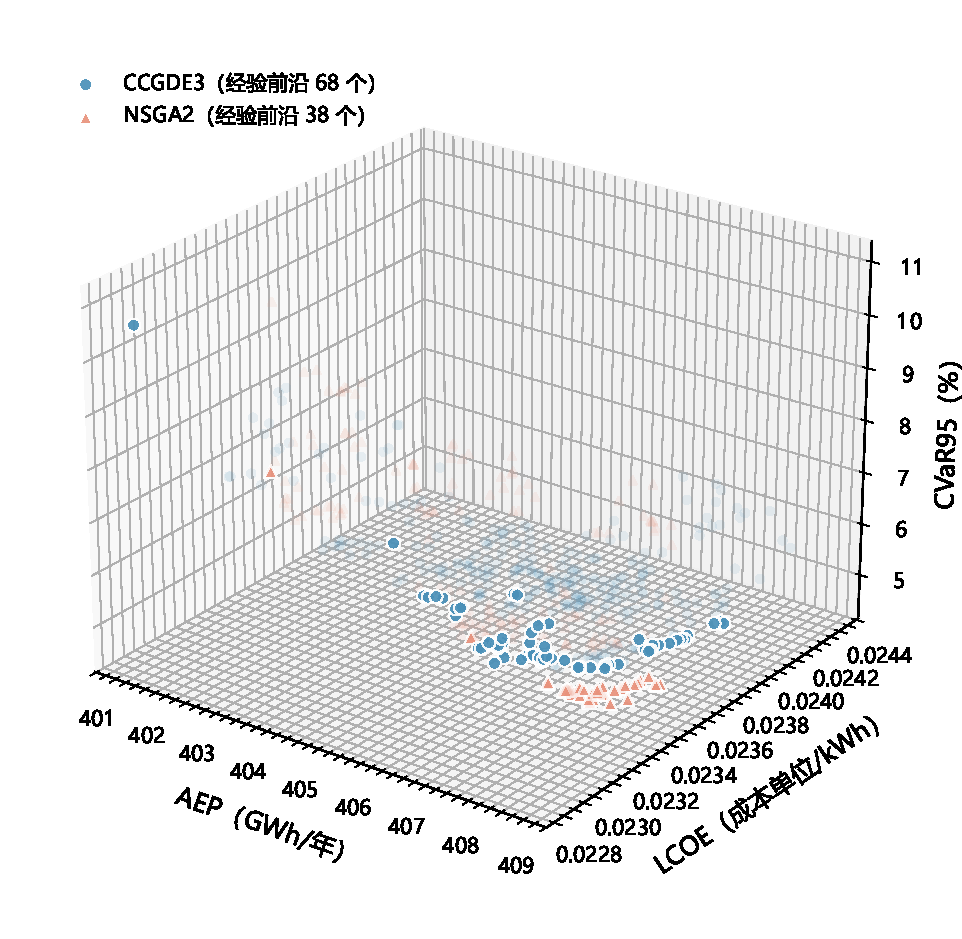
\includegraphics[width=0.88\textwidth]{图表/fig_continuous_pareto_front.pdf}
  \caption{连续坐标版两种算法的三目标最终解集与合并经验 Pareto 前沿。}
  \label{fig:continuous-pareto}
\end{figure}

\begin{figure}[H]
  \centering
  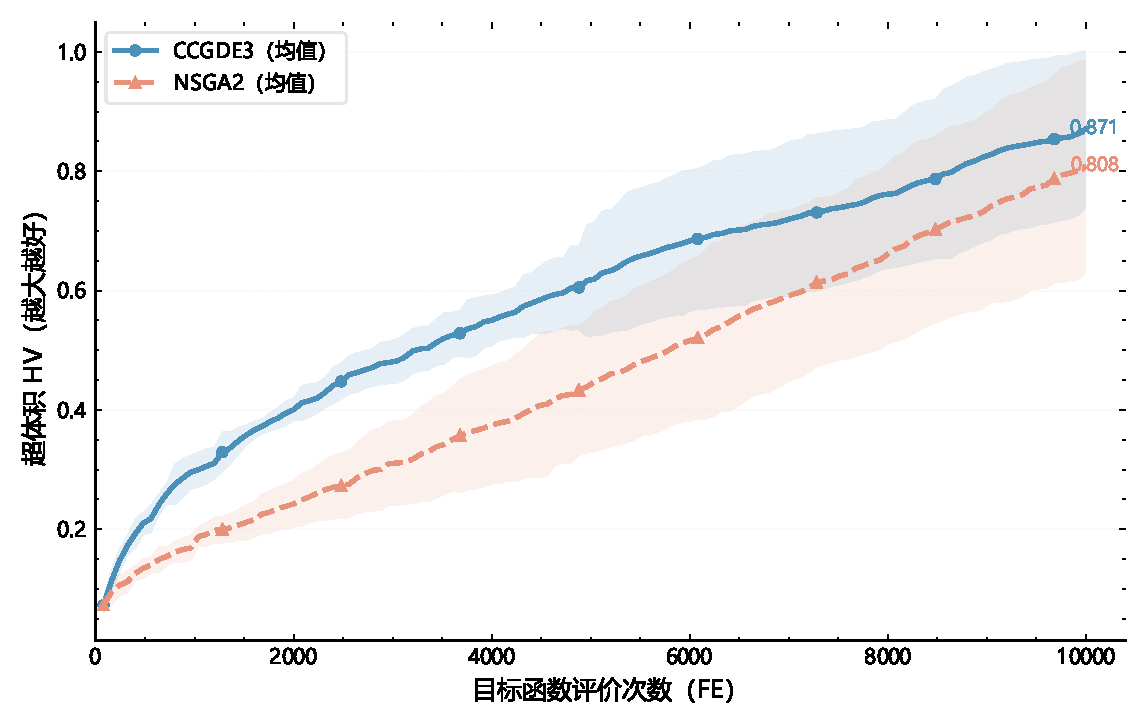
\includegraphics[width=0.84\textwidth]{图表/fig_continuous_convergence_hv.pdf}
  \caption{连续坐标版 HV 收敛过程。曲线为 5 次运行均值，阴影为均值$\pm$1倍标准差。}
  \label{fig:continuous-convergence}
\end{figure}

\begin{figure}[H]
  \centering
  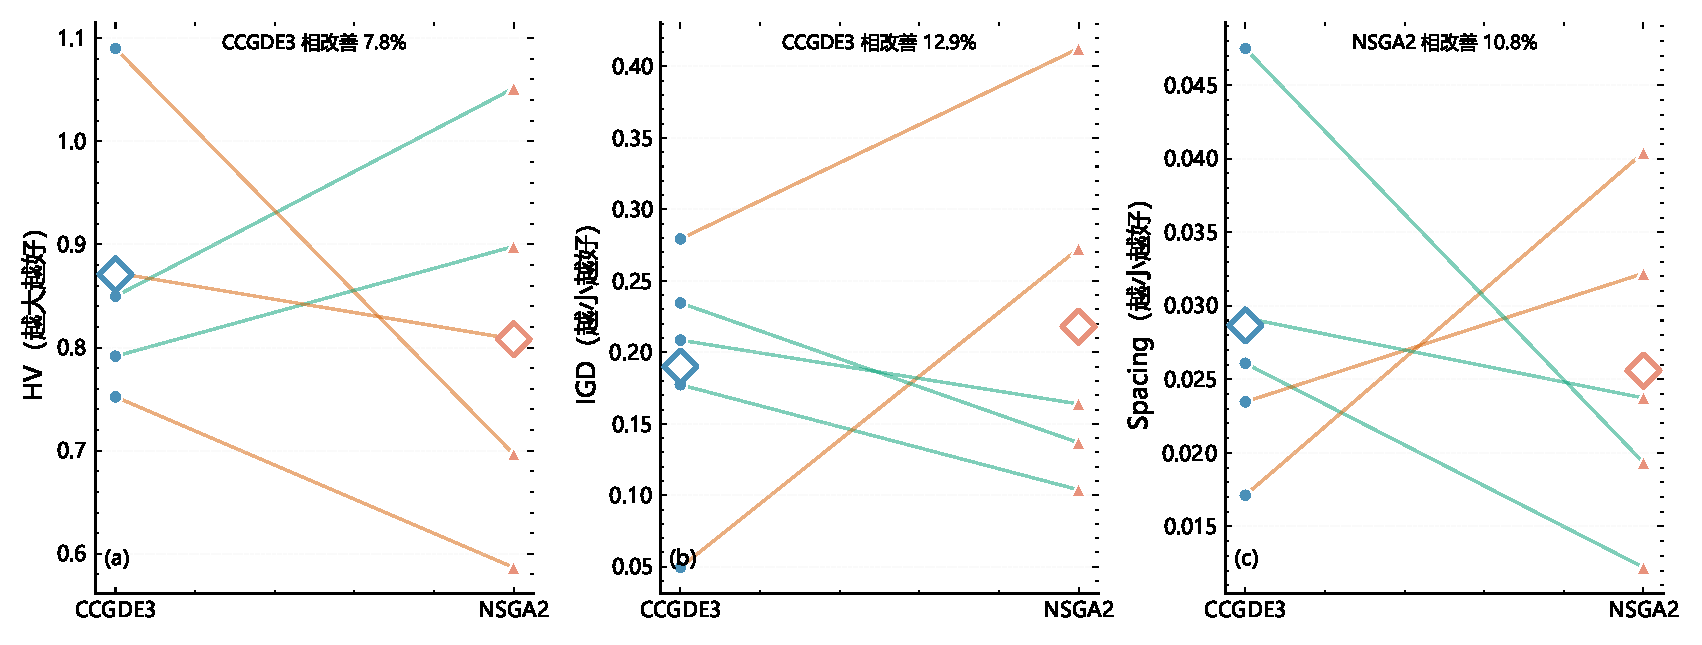
\includegraphics[width=\textwidth]{图表/fig_continuous_metric_distribution.pdf}
  \caption{连续坐标版 5 个随机种子下 HV、IGD 和 Spacing 的配对对比。}
  \label{fig:continuous-metrics}
\end{figure}

\begin{figure}[H]
  \centering
  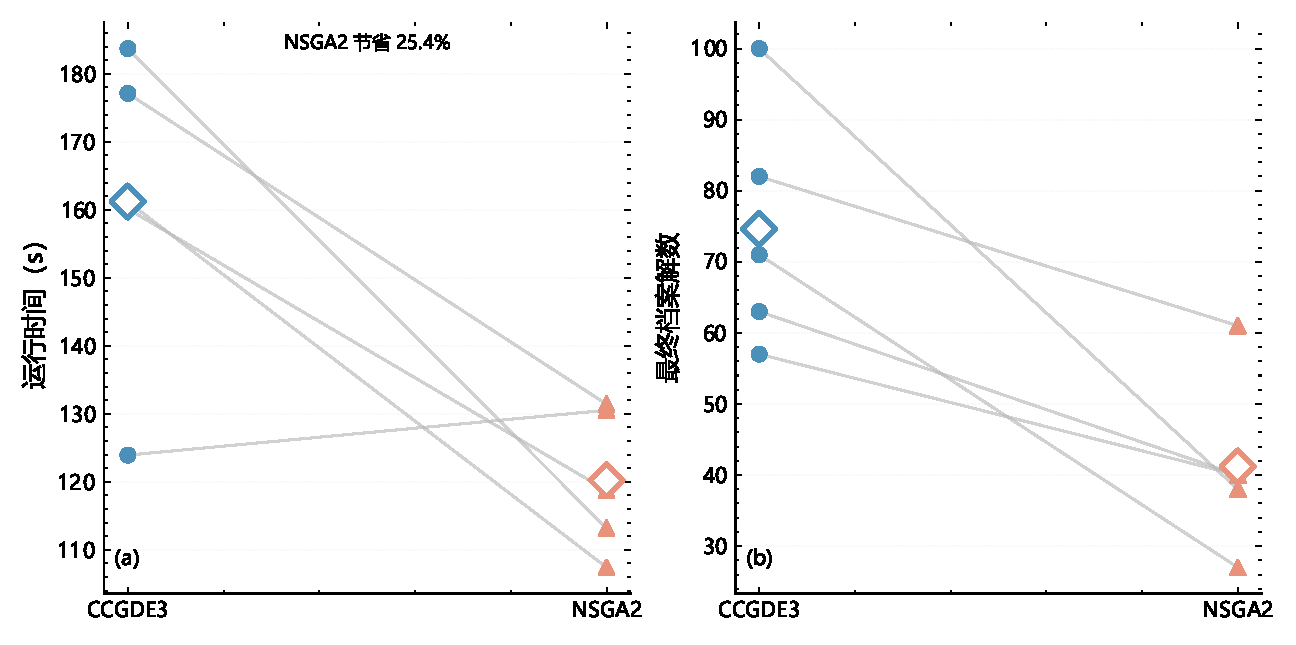
\includegraphics[width=0.90\textwidth]{图表/fig_continuous_runtime.pdf}
  \caption{连续坐标版的运行时间和最终档案规模。}
  \label{fig:continuous-runtime}
\end{figure}

\begin{figure}[H]
  \centering
  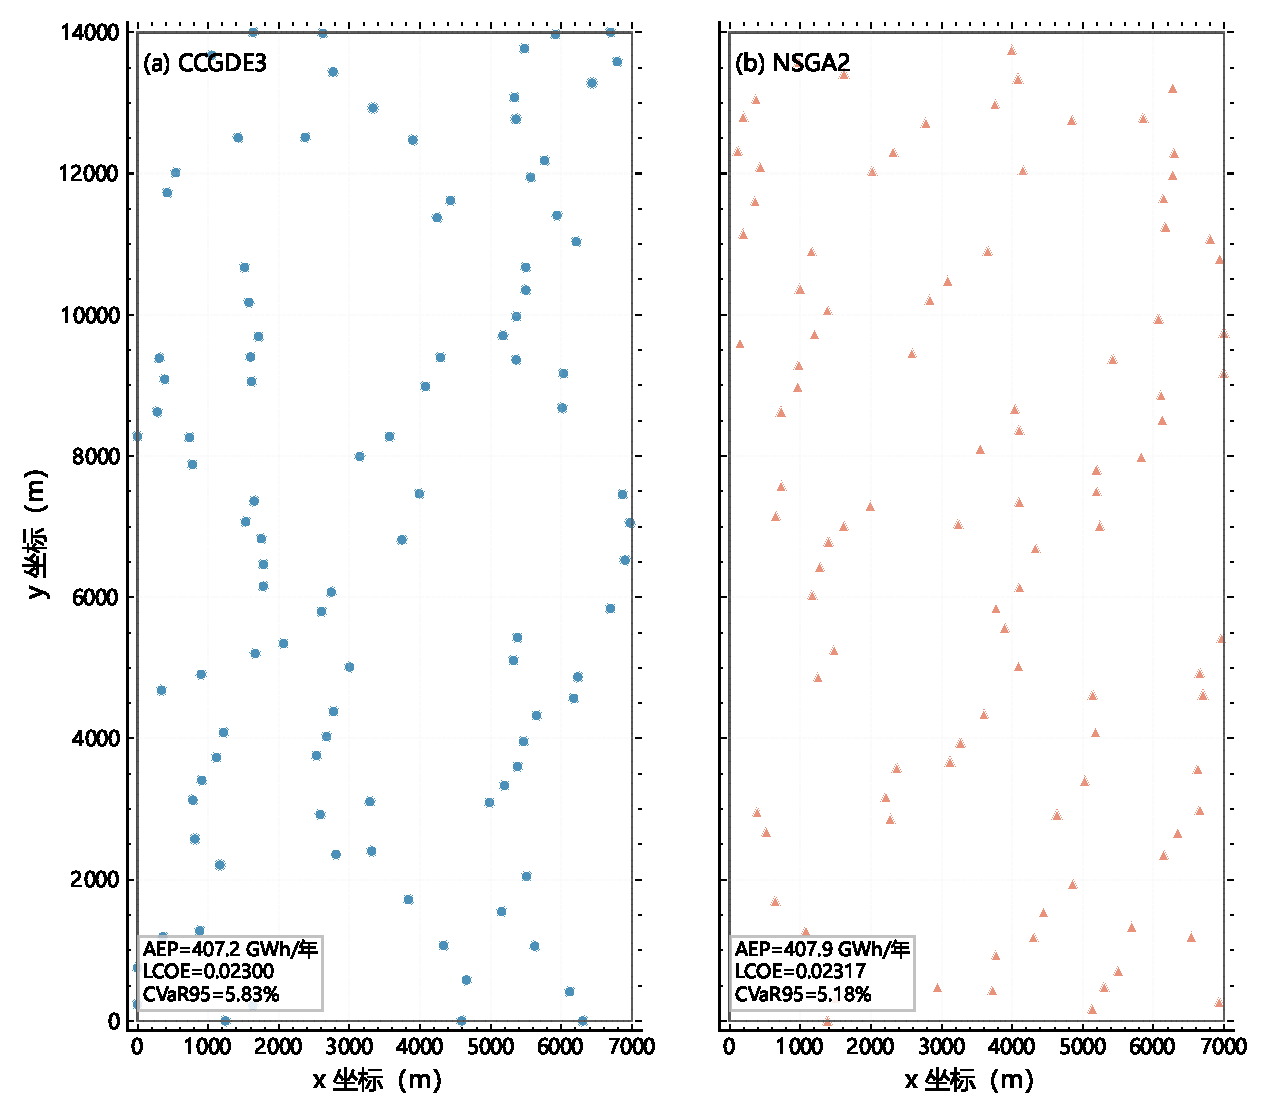
\includegraphics[width=0.90\textwidth]{图表/fig_continuous_layouts.pdf}
  \caption{连续坐标版两种算法代表性折中解的 100 台风机布局。}
  \label{fig:continuous-layouts}
\end{figure}

\begin{figure}[H]
  \centering
  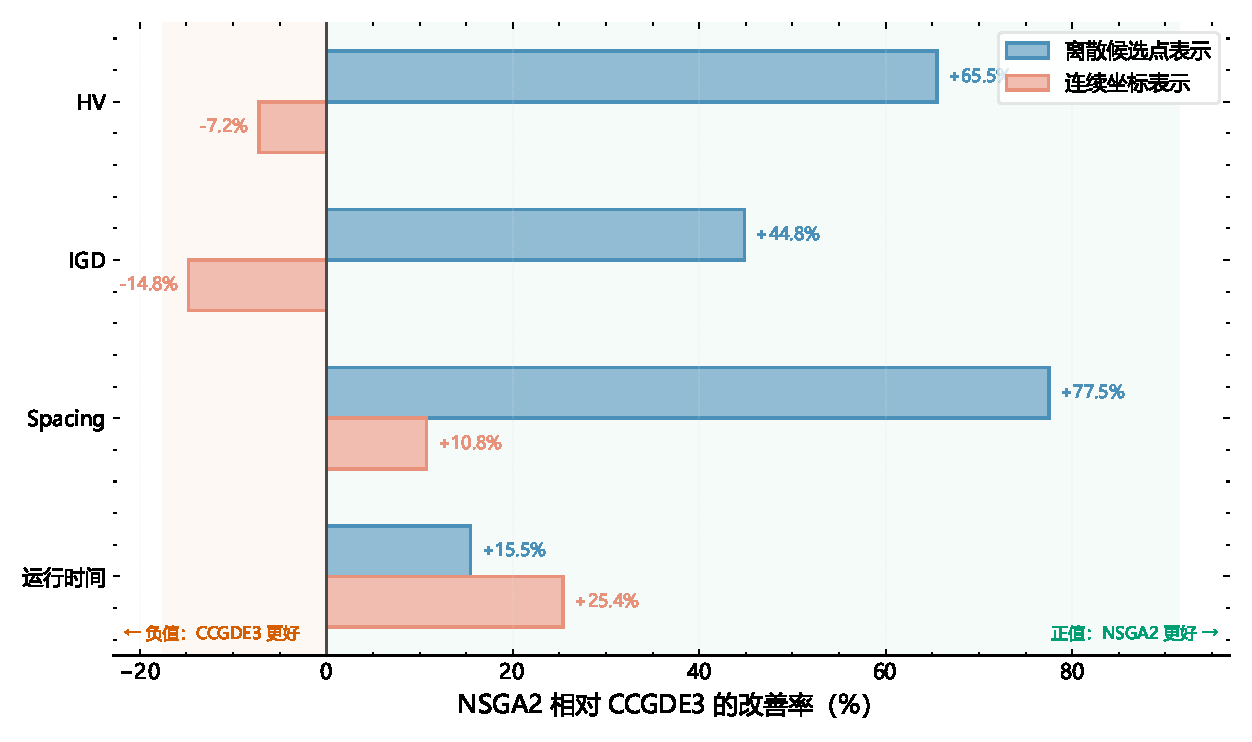
\includegraphics[width=0.92\textwidth]{图表/fig_representation_effect.pdf}
  \caption{离散候选点表示和连续坐标表示下，NSGA2 相对 CCGDE3 的指标改善率。}
  \label{fig:representation-effect}
\end{figure}

\begin{figure}[H]
  \centering
  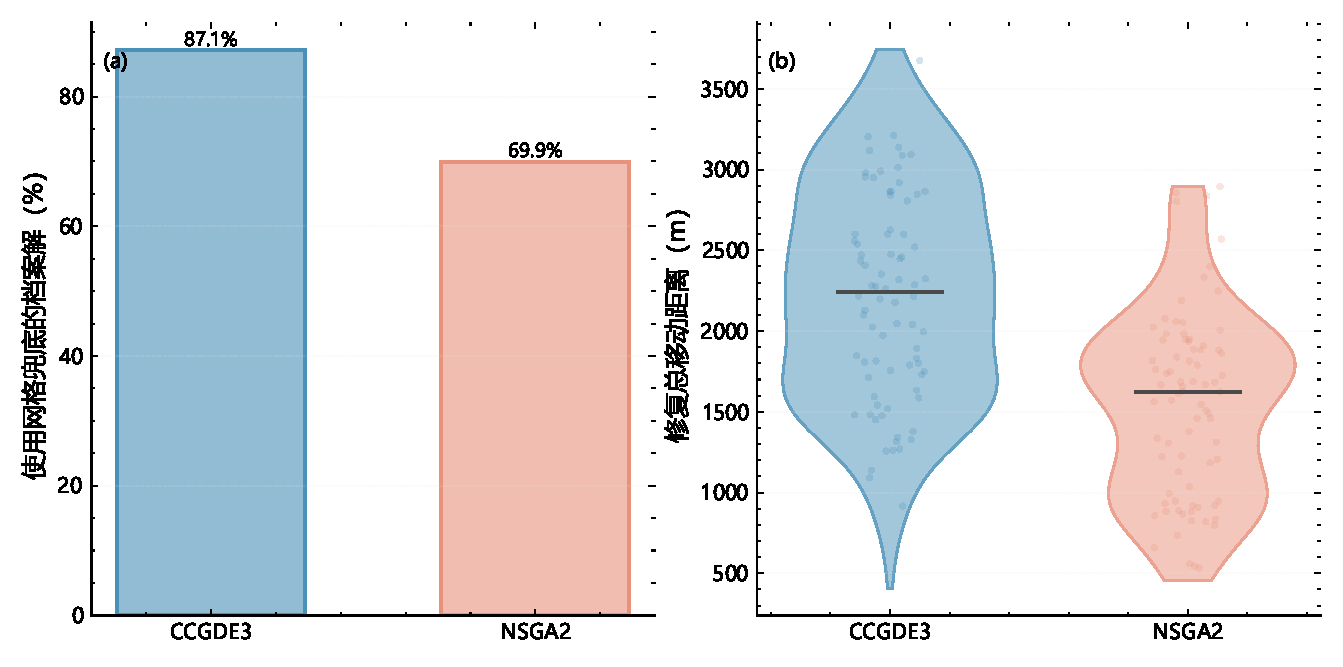
\includegraphics[width=0.92\textwidth]{图表/fig_continuous_repair_diagnostics.pdf}
  \caption{连续布局修复器诊断：网格兜底使用率与修复总移动距离分布。}
  \label{fig:continuous-repair}
\end{figure}

\clearpage
\begin{table}[H]
\centering
\caption{连续变量版算法性能对比（5次独立运行）}
\label{tab:continuous-comparison}
\begin{tabular}{lcccc}
\toprule
算法 & HV$\uparrow$ & IGD$\downarrow$ & Spacing$\downarrow$ & 时间/s$\downarrow$ \\
\midrule
CCGDE3 & 0.8712 $\pm$ 0.1312 & 0.1899 $\pm$ 0.0869 & 0.0287 $\pm$ 0.0114 & 161.22 $\pm$ 23.19 \\
NSGA2 & 0.8082 $\pm$ 0.1793 & 0.2179 $\pm$ 0.1259 & 0.0256 $\pm$ 0.0110 & 120.25 $\pm$ 10.57 \\
\bottomrule
\end{tabular}
\end{table}

\begin{table}[H]
\centering
\caption{连续变量版代表性折中解}
\label{tab:continuous-representatives}
\begin{tabular}{lcccc}
\toprule
算法 & 运行序号 & AEP/(GWh/\text{year}) & LCOE & CVaR95/(\%) \\
\midrule
CCGDE3 & 2 & 407.22 & 0.023000 & 5.83 \\
NSGA2 & 1 & 407.93 & 0.023167 & 5.18 \\
\bottomrule
\end{tabular}
\end{table}




